\documentclass[11pt,answers]{exam}

% Load useful packages
% Read in necessary packages
\usepackage{import}
\usepackage{amsmath}
\usepackage{amsfonts}
\usepackage{amssymb}
\usepackage{graphicx}
\usepackage{hyperref}
\usepackage{color}
\usepackage{subfigure}
\usepackage{tikz}

% Set various options for exam package
\shadedsolutions % defines the style of the solution environment

% Set lesson name, etc.
\newcommand{\coursename}{Math 312}
\newcommand{\lessonname}{Problem Set 6}
\newcommand{\duedate}{16 April 2016}
\newcommand{\names}{Ian Gallmeister, Kevin Fortune, Meridith Richmond, Elizabeth Ruvolo}

% Set headers/footers to look nice
\pagestyle{headandfoot}
\firstpageheader{\textbf{\large \coursename\ \lessonname}}{}{\textbf{\large Due \duedate}}
\firstpageheadrule
\runningheader{\textbf{\large \coursename\ \lessonname}}{}{\textbf{\large Due \duedate}}
\runningheadrule
\firstpagefooter{\names}{}{Page \thepage\ of \numpages}
\firstpagefootrule
\runningfooter{\names}{}{Page \thepage\ of \numpages}
\runningfootrule

% Define commands related to marking up content
\newcommand{\source}[1]{}

% Define commands related to general mathematical style
\renewcommand{\exp}[1]{e^{#1}}

\renewcommand{\theenumi}{(\textsc{\alph{enumi}})}
\renewcommand{\labelenumi}{\theenumi}
\renewcommand{\thequestion}{\arabic{question}}
\renewcommand{\questionlabel}{(\thequestion)}
%%%%%%%%%%%%%%%%%%%%%%%%%%%%%%%%%%%%%%%%%%%%%%%%%%%%%%%%%%%%

\begin{document}
\begin{questions}

\addtocounter{question}{42}
\item Plot the phase portrait and classify the following system: $\dot{x} = 5x + 10y, \: \dot{y} = -x - y$
\begin{solution}
\end{solution}


\item Plot the phase portrait and classify the following system: $\dot{x} = -3x + 2y \: \dot{y} = x - 2y$
\begin{solution}
Using \texttt{Eigensystem[]} in Mathematica, we find that the eigenvalues and eigenvectors are: $\displaystyle \lambda_1 = -1, \vec{v_1} = \binom{1}{1}, \:\: \lambda_2 = -4, \vec{v}_2 = \binom{-2}{1}$
\begin{center}
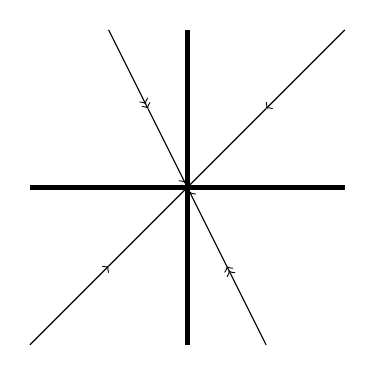
\begin{tikzpicture}
\draw[ultra thick] (0, -2) -- (0, 2);
\draw[ultra thick] (-2, 0) -- (2, 0);
\draw[->] (2,2) -- (1,1);
\draw[->] (1,1) -- (0,0);
\draw[->] (-2,-2) -- (-1,-1);
\draw[->] (-1,-1) -- (0,0);
\draw[->>] (-1,2) -- (-0.5,1);
\draw[->>] (-0.5,1) -- (0,0);
\draw[->>] (1,-2) -- (0.5,-1);
\draw[->>] (0.5,-1) -- (0,0);
\end{tikzpicture}
\end{center}
\end{solution}


\item Suppose we choose a linear system $\displaystyle \dot{x} = Ax, \: \left(\begin{array}{cc} a & b \\ c & d \end{array} \right)$ at random.  What are the probabilities of getting each type of fixed point.
\newline\textsc{(a)} Each matrix entry is drawn from a uniform distribution on $[-1, 1]$
\newline\textsc{(b)} Entries $a$ and $c$ are uniformly distributed on $[-1, 1]$, but $b$ comes from $[-0.5, 0.5]$ and $d$ is drawn out of $[0, 2]$
\newline\textsc{(c)} What if each entry is drawn from a normal distribution?
\begin{solution}
So, we did this in R because of its C backend to speed up otherwise interpreted stuff.  The script checked for saddles, unstable nodes and spirals, centers, stable nodes and spirals, nonisolated fixed points, and other.  There was also an error counter, but that never got above zero up.  The script is included at the end of the document.  All numbers are shown as a gross and a proportion.
\newline\textsc{(a)} For all elements drawn from \texttt{runif{min = -1, max = 1}}
\begin{verbatim}
#Results, {{a,b},{c,d}}, all from runif(4, min = -1, max = 1)
> c(saddle, saddle/100000000)
[1] 4.999005e+07 4.999005e-01
> c(unstable_node, unstable_node/100000000)
[1] 9.022835e+06 9.022835e-02
> c(unstable_spiral, unstable_spiral/100000000)
[1] 1.597933e+07 1.597933e-01
> c(center, center/100000000)
[1] 0 0
> c(stable_spiral, stable_spiral/100000000)
[1] 1.597992e+07 1.597992e-01
> c(stable_node, stable_node/100000000)
[1] 9.02786e+06 9.02786e-02
> c(nonisolated_fixed_point, nonisolated_fixed_point/100000000)
[1] 0 0
> c(stars_degenerate_etc, stars_degenerate_etc/100000000)
[1] 0 0
\end{verbatim}
\textsc{(b)} For a more biased matrix.
\begin{verbatim}
#Results, {{a,b},{c,d}}, a and c from runif24, min = -1, max = 1)
# b from runif(1, min = -0.5, max = 0.5) 
#d is drawn from runif(1, min = 0, max = 2)
> c(saddle, saddle/100000000)
[1] 4.998815e+07 4.998815e-01
> c(unstable_node, unstable_node/100000000)
[1] 3.374639e+07 3.374639e-01
> c(unstable_spiral, unstable_spiral/100000000)
[1] 1.415956e+07 1.415956e-01
> c(center, center/100000000)
[1] 0 0
> c(stable_spiral, stable_spiral/100000000)
[1] 1.534639e+06 1.534639e-02
> c(stable_node, stable_node/100000000)
[1] 5.71259e+05 5.71259e-03
> c(nonisolated_fixed_point, nonisolated_fixed_point/100000000)
[1] 0 0
> c(stars_degenerate_etc, stars_degenerate_etc/100000000)
[1] 0 0
\end{verbatim}
\textsc{(c)} Elements from normal distribution
\begin{verbatim}
> c(saddle, saddle/100000000)
[1] 4.999844e+07 4.999844e-01
> c(unstable_node, unstable_node/100000000)
[1] 1.035318e+07 1.035318e-01
> c(unstable_spiral, unstable_spiral/100000000)
[1] 1.464709e+07 1.464709e-01
> c(center, center/100000000)
[1] 0 0
> c(stable_spiral, stable_spiral/100000000)
[1] 1.464661e+07 1.464661e-01
> c(stable_node, stable_node/100000000)
[1] 1.035468e+07 1.035468e-01
> c(nonisolated_fixed_point, nonisolated_fixed_point/100000000)
[1] 0 0
> c(stars_degenerate_etc, stars_degenerate_etc/100000000)
[1] 0 0
\end{verbatim}
\end{solution}


\item Do opposites attract?  Analyze $\dot{R} = aR + bJ, \: \dot{J} = -bR -aJ$
\begin{solution}
This problem can be rewritten as $\dot{x} = Ax$ where $x = \binom{R}{J}$ and $\displaystyle A = \left(\begin{array}{cc} a & b \\ -b & -a \end{array}\right)$
This gives us $\Delta = -a^2 + b^2$ and $\tau = 0$, so this function's fixed point is a center.  The eigenvalues and eigenvectors are $\lambda_1 = \sqrt{a^2 + b^2}, \vec{v}_1 = \binom{-(a - \sqrt{a^2 + b^2})/b}{1} \hbox{ and } \lambda_2 = -\sqrt{a^2 + b^2}, \vec{v}_2 = \binom{-(a + \sqrt{a^2 + b^2})/b}{1}$
\end{solution}


\end{questions}

R Script:
\begin{verbatim}
#Monte Carlo Sim
#100,000,000 Matrices - classify fixed points

0 -> saddle
0 -> unstable_node
0 -> unstable_spiral
0 -> center
0 -> stable_spiral
0 -> stable_node
0 -> nonisolated_fixed_point
0 -> stars_degenerate_etc
0 -> this_is_embarrasing
0 -> done_fucked_up

for(i in 1:100000000){ #Hundred Million Matrix Runs
  #twobytwo <- matrix(data = runif(4, min = -1, max = 1), nrow = 2, ncol = 2)
  #twobytwo <- matrix(data = c(runif(2, min = -1, max = 1), 
            runif(1, min = -0.5, max = 0.5), runif(1, min = 0, max = 2)), 
            nrow = 2, ncol = 2, byrow = FALSE) #biased
  twobytwo <- matrix(data = c(rnorm(4, mean = 0, sd = 0.5)), 
            nrow = 2, ncol = 2) #normal
  determinant <- twobytwo[1,1]*twobytwo[2,2] - twobytwo[1,2]*twobytwo[2,1]
  trace <- twobytwo[1,1] + twobytwo[2,2]
  if(determinant < 0){
    saddle <- saddle + 1 #Saddle is only det > 0
  } else if(determinant == 0){nonisolated_fixed_point <- 
        nonisolated_fixed_point + 1 #Nonisolated fp is the only det = 0 case
  } else if(determinant > 0){ # For all the det > 0
      if(trace == 0){center <- center + 1 #Trace = 0 --> center
    } else if((trace*trace - 4*determinant) == 0){stars_degenerate_etc <- 
            stars_degenerate_etc + 1 #Thingy = 0 --> stars,degenerate, etc...
    } else if(trace < 0){ #Trace less than zero
        if((trace*trace - 4*determinant)  > 0){stable_node <- 
                stable_node + 1 #Thingy less than zero --> stable spiral
        } else if((trace*trace - 4*determinant) < 0){stable_spiral <- 
                stable_spiral + 1 #Thingy greater than zero --> stable node
        } else{this_is_embarrasing <- this_is_embarrasing + 1} 
            #If neither stable spiral nor stable node, code done fucked up
    }
    else if(trace > 0){ #If trace greather than zero
        if((trace*trace - 4*determinant)  > 0){unstable_node <- 
                unstable_node + 1 #Thingy less than zero --> unstable spiral
      } else if((trace*trace - 4*determinant) < 0){unstable_spiral <- 
                unstable_spiral + 1 #Thingy greater than zero --> unstable node
      } else{this_is_embarrasing <- this_is_embarrasing + 1} 
                #If neither stable spiral nor stable node, code done fucked up
    }
    else{done_fucked_up <- done_fucked_up + 1} #First nesting fuckup
  }
}
\end{verbatim}
\end{document}